\documentclass[a4paper,english]{ifimaster}

\usepackage[utf8]{inputenc}
\usepackage{babel,duomasterforside}
\usepackage{csquotes}
\usepackage{hyperref}

\usepackage[backend=biber,style=authoryear]{biblatex}
\addbibresource{bibliography.bib}





\title{Learning}
\subtitle{Subtitle}
\author{Mathias Kirkerød}

\begin{document}
\duoforside[dept={Department of Informatics},
program={Informatics: Language and Communication},
long]

\frontmatter{}
\chapter*{Abstract}

\tableofcontents{}
\listoffigures{}
\listoftables{}

\chapter*{Preface}

\mainmatter{}






















\part{Introduction}
\chapter{Introduction}
	\section{Background and Motivation}
	\subsection{Introduction REM}
	\textbf{Cancer}
	Cancer is, today, the second leading cause of death in the world, only behind cardiovascular diseases.\\  %TODO CITE
	It is one of the leading causes of mortality worldwide, with approximately 14 million new cases in 2012. %TODO  "http://www.who.int/mediacentre/factsheets/fs297/en/ World Health Organization. February 2018. Retrieved 19 April 2018.
	It is defined as a disease that has an abnormal cell growth with the potential to spread into other parts of the body.%TODO https://www.cancer.gov/about-cancer/understanding/what-is-cancer
	In contrast to many other diseases cancer does not start from a foreign entity (such as a bacteria or virus), but it is often from a malfunctioning cell that starts dividing rapidly. 
	This can happen when a cell is damaged, by for instance by radiation, and the resulting damage causes the cell to uncontrollably divide. 
	Especially in the later part of life everyone has the chance of getting cancer, and in fact everyone does. Our own body is designed to detect and remove cells that are prone
	to divide uncontrollably. Unfortunately this system is not perfect, and the immune system can in some cases overlook cells that are cancerous.
	
	
	
	\vspace{10px}
	
	\subsection{Statistics on cancer REM}
	The western (or modern) world has been in a battle against cancer, and despite a 
	lot of new cures/innovations it is still one of the deadliest killers in the world. 

	
	\textit{The most common types of cancer in males are lung cancer, prostate cancer, colorectal cancer and stomach cancer.\cite{stewart2014world}}
	
	
	\vspace{10px}
	\subsection{colorectal cancer REM}
	You can get cancer in every major organ, but some types of cancer are more common than others.
	For instance cancer in the gastrointestinal tract (GI) is one of the more common places 
	to get cancer. This is just behind x, and it has a mortality rate of x in the first y years. %TODO CITE 
	We often call this 5 year survival rate for z. This is the standard way to measure the life expectancy of a patient diagnosed with cancer. 
	
	
	\vspace{10px}
	\subsection{polyps REM}
	The colorectal cancer often starts in polyps. 
	Polyps are, polyps do.\\
	
	\vspace{10px}
	\subsection{preventative matters and early detection REM}
	\textit{-colonoscopy\\ 
		-mri\\
		-pillcam\\}
	A good way to fight cancer is to detect and remove it early, or some times remove areas with a high chance of getting cancer.
	We classify cancer in to x stages, and the stage the patient are in often determines the chance you have for survival. 
	In general, the earlier you find the cancer, the more likely it is that the patient will survive. 
	And as mentioned above, the colorectal cancer often starts in these polyps. A crucial stage to prevent cancer lies in the 
	early removal of there polyps.
	Reports shows x about this %TODO find Reports
	
	*4 stages maybe?
	*early detection
	*survival rate
	
		
	Because of this the ability to find, and remove colorectal polyps is great for preventing cancer in the GI tract. 
	
	
	\vspace{10px}
	\textbf{colonoscopy/Ontonoscopy}
	In the most common way to look for polyps in the GI tract is to use a medical team, and perform a colonoscopy or Ontonoscopy
	colonoscopy is preformed with a camera.....\\
	Onoskopy is the same procedure, only the camera is inserted orally. \\
	\textbf{Advantages}
	  * Accurate 
	  *
	\vspace{10px}
	\textbf{Disadvantages}
	  *expensive 
	
	\vspace{10px}
	\textbf{MRI}
	
	\vspace{10px}
	\textbf{pillcam}
	
	In the last 3-4 years there have been testing and development on the pillcam project EIR. Machine learning has, through 
	many of the earlier projects, got the detection rate for the polyps up to x\% %TODO cite
	
	
	\vspace{10px}
	\subsection{Simulas contribution to the pillcam project REM}
	Simulas EIR
		

		
	* CAD ACD (computer aided diagnosis, Automated computer diagnosis)
	
	\section{Goal / Problem}
		\subsection{pillcam project has lots of data, can be used to train an unsupervised network REM}
		\subsection{Use Unsupervised learning as a pre-processing tool REM}
		\subsection{use Unsupervised-NN/GAN for image enhancements so that a NN can train better REM}
		* Now that we got a lot of tests, why not unsupervised
		As mentioned, simula research centre has done a lot of testing on the pillcam project.
		  
		* We know that we can get some results using a neural network
		* Can this be done unsupervised?
		* Can it be done in a fashion that is better than S-ML
		 
		 REM

		
	\section{Scope and Limitations}
		\subsection{Use Unsupervised NN to find polyps REM}
		\subsection{Use Unsupervised NN for pre-processing REM}
		* Something about earlier research already got far, so the scope is mainly unsupervised deep learning.
		* (and how to generalise it?)
*REMegression	
		

	\section{Research method}
	\section{Related work}
	\section{Outline}
	The rest of the thesis is structed as follows:
	
	\textbf{Chapter 2 - Background}\\
	*talk about cancer
	*talk about machine learning.
	*how to use ML on the pillcam video?
	\textbf{Chapter 3 - Me doing stuff}\\
	\textbf{Chapter 4 - Me got and present result}\\
	\textbf{Chapter 5 - Me saying result was good A+}\\
	
	
\chapter{Background}
	\section{Cancer and polyps}
	  \subsection{What we are looking for REM}
	  Different types of disorders.
	  %TODO image of polyp
	  Polyp is harmless, but if left untreated it can become cancerous
	  %TODO tell the risk
	  Pictures is from the pillcam project, kvasir dataset.
	  \subsection{images from pillcam, and what we are looking at/for REM}
	  %TODO More pictures of polyps, and other anomalies
	  
	
	\section{Naive Methods REM}
	  Now that we have an idea of what we are looking for we can first turn to some more naive methods for detecting anomalies, and for enhancing the images.\\
	  The field of image processing has been researched since\\ %TODO WHEN
	  
	  Using some of the classic methods in image processing we can see if\\ %TODO
	  
	  We often describe the method in to two groups of information: First and Second order statistics.\\
	  \textbf{First order:} First order statistics does not take in to account the relative positioning of the pixels in the image, and because of this, gives much less
	  information than the second order statistics.\\
	  Example of First order statistics is often what information we can get out of a histogram. This can be scewness, variance, and mean value.\\
	  
	  \vspace{10px}
	  
	  \textbf{Second order:} Second order statistics takes in to account the relative positioning of the pixels in the image. We can calculate the GLCM matrix and get a much more detailed 
	  view of the image. \\
	  
	  
	  
	  \subsection{GLCM}
	    A GLCM (Grey-level co-occurrence matrix) is a matrix that is used when examining the spatial relationship of pixels in a texture. 
	    The calculation of a GLCM gives us how often pairs of pixels with spesific values and a specified spatial relationship occur at a given place in an image. %TODO CITE
	  
	    \subsubsection{Algorithm}
	      For simplicity we use only greyscale in this example:
	      \begin{figure}[h]
		\centering
		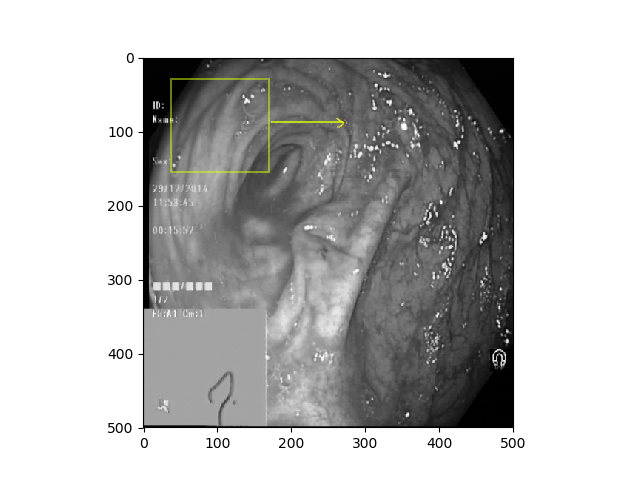
\includegraphics[scale=0.5]{figures/sliding_window_box.png}
		\caption{GLCM capturing features}
	      \end{figure}
	      The algorithm starts by running a sliding window over the image, often with a stride, and for each stops calculates the spatial relationship between each pixel specified.
	      The result can be something like this figure %TODO link to figure
	      where we can read out the most likely neighbouring pixel.
	       \begin{figure}[h]
		\centering
		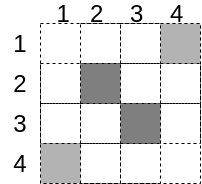
\includegraphics[scale=0.5]{figures/Simple_GLCM.png}
		\caption{GLCM Matrix}
	      \end{figure}
	      The darker colours on in the matrix is indicating that we often have a jump between, for instance pixel-value of 1 and a pixel-value of 4, but no from 1 to 1.\\
	      With this information we can get a naive pattern-recogniser. 
	    \subsubsection{Other uses}
	      Besides for the pattern recognition we can use the GLCM to get the information on:
	      \begin{itemize}
	       \item \textbf{Contrast} is the difference in luminance or colour in the picture. We would expect low contrast in the “background” and higher contrast around edges and irregular objects.
	       \item \textbf{Homogeneity} is how similar a local area is to itself
	       \item \textbf{Variance} $\sigma^2$ , is directly a measure of ”roughness”
	       \item \textbf{Mean} value of a GLCM can give us areas with higer or lower pixel values. Good way to find polyps if they are lighter than the tissue around.
	       \item \textbf{Entropy}
	       \item \textbf{Energy}
	      \end{itemize}


	  
	  \subsection{Edge detection}
	    Using Edge detection in is another viable way to look for polyps. 
	    \begin{figure}[h]
	      \centering
	      \begin{minipage}[b]{0.45\textwidth}
		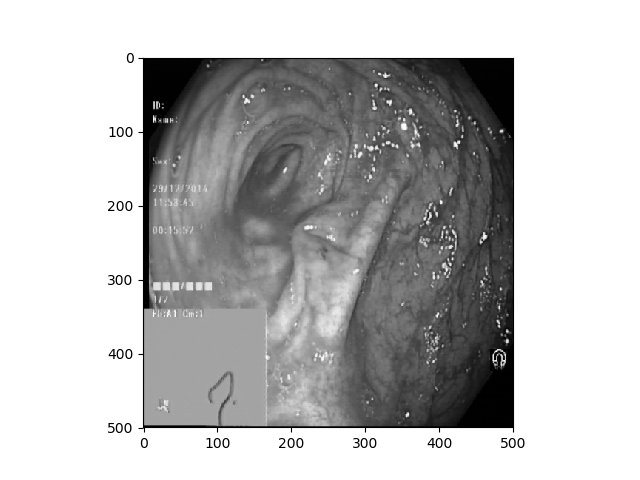
\includegraphics[width=\textwidth]{figures/sliding_window.png}
		\caption{Original image}
	      \end{minipage}
	      \hfill
	      \begin{minipage}[b]{0.45\textwidth}
		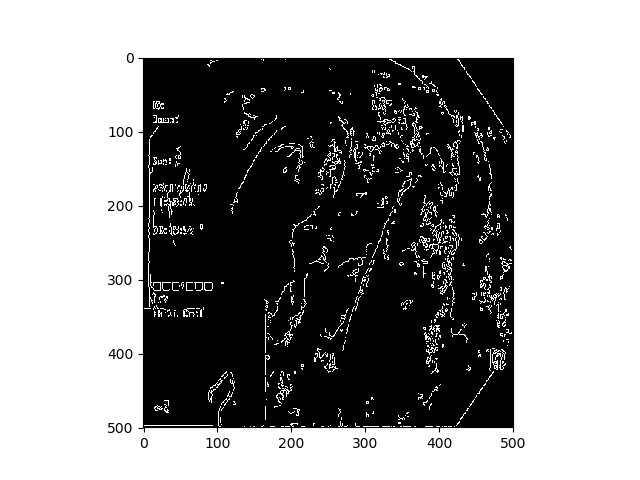
\includegraphics[width=\textwidth]{figures/Canny.png}
		\caption{Edges of the picture}
	      \end{minipage}
	    \end{figure}
	    \subsubsection{Algorithm}
	      For each pixel look at the neighbouring pixel, if \\
	      
	      \begin{centering} 
		$ abs(p_a - p_b)>tresh $\\ 
	      \end{centering}
	      
	      then mark pixel as an edge pixel. \\
	      
	  \subsection{Hough Transforms}
	    Using for instance Canny edge detection %TODO CITE
	    we can get a better view of where the potential border of the polyp/anomaly is. (As shown in %TODO FIG CITE)
	    
	    A hough transform can i theory have many/any shape(s), and together with edge detection, we might find some of the polyps this way.
	    
	    
	  
	  
	\section{Machine Learning}
	Machine learning is a very broad term, but can i short be summarised by:\\
	\vspace{10px}
	
	\textit{ A computer program is said to learn from experience E with respect to 
	some class of tasks T and performance measure P, if its performance at
	tasks in T, as measured by P, improves with the experience E. } 
	\cite{MitchellTomM1997Ml}\\
	
	\vspace{10px}
	Here we have a couple of parameters:\\
	\textbf{E} text about p\\
	\textbf{T} text about p\\
	\textbf{P} text about p\\
	
	From this we see that the goal of machine learning is to improve some performance P with experience.
	\textbf{might here talk about different tasks ML can do?}
	
	  \subsection{Supervised \& Unsupervised machine learning}
	  We often divide machine learning in to two (diffuse) categories: supervised and unsupervised.\\
	  \textbf{Supervised learning:} is the act of training with data that has an answer or a label. The learning algorithm can get supervision while 
	  training on the task. An example on a supervised task  is to recognise handwritten numbers, or differentiate between dogs and cats. The task is supervised if the images
	  comes with the correct label in the data set. These  examples are typical classification examples, where the task is to identify the right group to classify the data to %TODO more
	  A simpler classification assignment is binary classification, where the target is (often) yes or no. Examples for binary classification is if an email is spam or not, is a car Norwegian 
	  or International. 
	  In the last example the classification changes from binary to multi-class if you sort the cars on every nationality, and not just Norwegian/non-Norwegian.
	  
	  Another type of supervised learning is regression. This is the act of prediction given prior data. Examples of regression is everything from prediction of stock prices, to house prices 
	  in an area, to\\ %TODO more
	  \begin{figure}
	     \centering
	    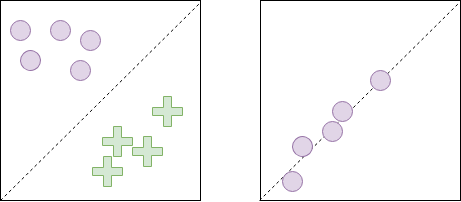
\includegraphics[scale=0.5]{figures/class_vs_reg.png}
	     \caption{Left: Example of binary classification. Right: Example of regression} 
	  \end{figure}

	  
	  \textbf{Unsupervised learning:} is the act of training without any supervision, on the sense that we do not give the algorithm the answer
	  to the training data set. %TODO more 
	 
	  Since we do not have categorised data in unsupervised learning, we often %TODO more
	  Types of unsupervised learning can for instance be clustering, the act of sorting data based on similarity. An example of this can be if you want to sort plants based on species, or 
	  you are detecting anomalies in a dataset.
	  Unsupervised learning can be used for PCA %TODO CITE 
	  or other dimensionaly reduction methods.\\
	  
	  A third method to used unsupervised learning is the adversarial route, where you use machine learning to make similar looking data to the original data set. 
	    
	   \begin{figure}
	     \centering
	    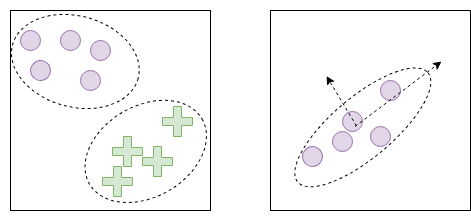
\includegraphics[scale=0.5]{figures/cluster_pca.png}
	     \caption{Left: Example of binary clustering. Right: Example of principal component analysis} 
	  \end{figure}

	 
	  In the description of supervised vs unsupervised we looked at a specific branch of machine learning: Classification. Classification is, as the name implies, the task of 
	  getting data sorted in to groups of similarity. 
	  
	  
	  \begin{itemize}
	    \item subsfication
	    \item r to the pillcam projression 
	    \item transcription/translation
	    \item de-noising /finding missing inputs
	  \end{itemize}
	  
	  Now that we have the definintion of machine learning we focus on the task at hand; finding polyps. In an ideal world we have a
	  Classification problem with only two classes: Non-polyp and polyp. 
	  
	  \begin{itemize}
	    \item SVM 
	    \item CNN 
	    \item random forests
	    \item knn
	  \end{itemize}
	  
	  \subsection{CNN}
	  \subsubsection{UCNN?}
	  
	  
	  
	  
	  
	
	
	
	
	  \subsection{Tasks (other better word goes here)}
\label{chap:Tasks}

\subsection{The rate of success}
What is a good result, how to measure?\\
\textbf{FP,TN,FN,TP}\\


%\subsection{deep vs shallow}		
\section{supervised vs unsupervised}
What it means to be S/US.\\
Something about the kind of experience allowed during the learning process.


\section{Unsupervised}
noe med å dele i grupper?
Experience the dataset containing many features, and finds useful properties of the structures. 
\textit{\textbf{Unsupervised learning algorithms} experience a dataset containing manyfeatures, then learn useful properties of the structure of this dataset. In the contextof deep learning, we usually want to learn the entire probability distribution thatgenerated a dataset, whether explicitly, as in density estimation, or implicitly, fortasks like synthesis or denoising. Some other unsupervised learning algorithmsperform other roles, like clustering, which consists of dividing the dataset intoclusters of similar examples.}
\cite{Goodfellow-et-al-2016}


\subsection{Approaches to unsupervised learning}
look at the \autoref{chap:Tasks} to see what applies to the unsupervised.

\subsection{Deep Unsupervised learning}
\subsection{more}
\section{Related work}


	      
		
		
		
		
		
		
		
		
		
		
		
		
		
		
		
		
		
		
		
		
		
		
		
		
		
\part{The project}

\chapter{Planning the project}
\section{Using Generative Adversarial Networks for enhancement and prediction}
Generative Adversarial Networks (GAN) was proposed by Goodfellow in 2014. \cite{GoodfellowGAN} %TODO fix cite
GANs is a specialised network consisting of generally two neural networks working against each other. 
The two networks are often called discriminator and generator. The generators job is to make data similar to the training data, and discriminator has the job if finding fake (generated) data.
%TODO insert picture here?

The GAN presented by Goodfellow 2014\cite{GoodfellowGAN} is a simple adversarial network, and it needs to be built upon to be used. Since we are working with images it is more suitable to use
DC-GAN instead. 

\subsection{DC-GAN}
  DC-GAN is a type of an Adversarial Network that still uses the adversarial approach, like the original GAN, but the two networks are deep convolutional networks. DC-GANs.
\subsection{CC-GAN}
  removing green squares

\section{Training an autoencoder to help the GAN}
An autoencoder (AE) is another form of a machine learning network. The autoencoders task is to  

\part{Conclusion}

\chapter{Results}

\backmatter{}

\printbibliography

\end{document}
